%=========================================================
\chapter{Modelo de la interacción}	
\label{cap:modInteraccion}

	Este capítulo presenta el diseño propuesto de las interfaces de usuario del sistema. Describiremos la estructura, disposición de elementos y flujo de interacción de las interfaces, así como los aspectos visuales como colores, tipografía y elementos gráficos.

\section{Modelo de navegación}

	La navegación entre pantallas se muestra en la figura~\ref{fig:mapa}. en el se explica ...

\begin{figure}[htbp]
	\begin{center}
		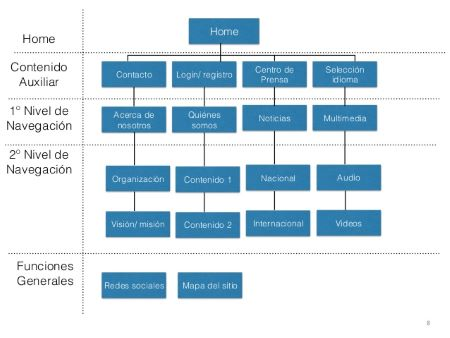
\includegraphics[width=.5\textwidth]{images/mapa}
		\caption{mapa}
		\label{fig:mapa}
	\end{center}
\end{figure}


%--------------------------------------
\section{IU1 Pantalla principal nutriologo}

\subsection{Objetivo}
	Permite al {\bf nutriologo} acceder a las principales funciones que tiene dentro del sistema

\subsection{Diseño}
	Esta pantalla \IUref{IU1}{Pantalla principal nutriologo} (ver figura~\ref{IU1}) aparece una vez que el usuario ha ingresado al sistema. 
 en la parte superior aparecen tres opciones de que acciones puede realizar el actor las cuales son {\bf añadir comida}, {\bf ver menú}, {\bf Cerrar Sesión}. 

 
%\IUfig[numero que modifica el tamaño de la imagen]{nombre de la imagen}{Id interfaz}{nombre interfaz.}
\IUfig[.7]{inicionutriologo}{IU1}{Pantalla principal nutriologo.}

\subsection{Salidas}

	Ninguna.

\subsection{Entradas}

        Ninguna.

\subsection{Comandos}
\begin{itemize}
	\item \IUbutton{Añadir comida}: muestra la \IUref{IU14}{Registrar comida}.
	\item \IUbutton{ver menú}: Muestra el menu de comidas de todo el mes
        \item \IUbutton{Cerrar sesión}Termina la sesion del usuario y lo saca del sistema
\end{itemize}

\subsection{Mensajes}
Ninguno.


\newpage
%--------------------------------------
\section{IU2 Pantalla principal medico}

\subsection{Objetivo}
	Permite al {\bf medico} acceder a las principales funciones que tiene dentro del sistema

\subsection{Diseño}
	Esta pantalla \IUref{IU2}{Pantalla principal medico} (ver figura~\ref{IU2}) aparece una vez que el usuario ha ingresado al sistema. 
 en la parte superior aparecen dos opciones de que acciones puede realizar el actor las cuales son {\bf Registrar incidente}, {\bf cerrar sesión}. 

 
%\IUfig[numero que modifica el tamaño de la imagen]{nombre de la imagen}{Id interfaz}{nombre interfaz.}
\IUfig[.7]{iniciomedico}{IU2}{Pantalla principal medico.}

\subsection{Salidas}

	Ninguna.

\subsection{Entradas}
        Ninguna.

\subsection{Comandos}
\begin{itemize}
	\item \IUbutton{Registrar incidente}: muestra la \IUref{IU20}{Incidencia médica}.
        \item \IUbutton{Cerrar sesión}Termina la sesion del usuario y lo saca del sistema
\end{itemize}

\subsection{Mensajes}

            Ninguno.

\newpage
%--------------------------------------
\section{IU3 Pantalla principal profesor}

\subsection{Objetivo}
	Permite al {\bf profesor} acceder a las principales funciones que tiene dentro del sistema

\subsection{Diseño}
	Esta pantalla \IUref{IU3}{Pantalla principal profesor} (ver figura~\ref{IU3}) aparece una vez que el usuario ha ingresado al sistema. 
 En la parte superior aparecen seis opciones de que acciones puede realizar el actor las cuales son: {\bf registrar ingesta}, {\bf registrar actividades}, {\bf Registrar tareas}, {\bf Registrar reporte}, {\bf Tomar asistencia}, {\bf Cerrar Sesión}. 

 
%\IUfig[numero que modifica el tamaño de la imagen]{nombre de la imagen}{Id interfaz}{nombre interfaz.}
\IUfig[.55]{iniciodocente}{IU3}{Pantalla principal profesor.}

\subsection{Salidas}

	Ninguna.

\subsection{Entradas}
        Ninguna.

\subsection{Comandos}
\begin{itemize}
	\item \IUbutton{Registrar ingesta}: muestra la \IUref{IU16}{Registrar ingesta}.
        \item \IUbutton{Registrar actividades}: muestra la \IUref{IU17}{Registrar actividades}.
        \item \IUbutton{Registrar tareas}: muestra la \IUref{IU18}{Registrar tareas}.
        \item \IUbutton{Registrar reporte}: muestra la \IUref{IU23}{Registrar reporte}.
        \item \IUbutton{Tomar asistencia}: muestra la \IUref{IU22}{Tomar asistencia}.
        \item \IUbutton{Cerrar sesión}Termina la sesion del usuario y lo saca del sistema
\end{itemize}

\subsection{Mensajes}

\begin{Citemize}
	\item Error al verificar los datos de acceso, vuelva a intentarlo.
\end{Citemize}


\newpage
%--------------------------------------
\newpage
\section{IU4 Pantalla principal Recursos Humanos}

\subsection{Objetivo}
	Permite a {\bf Recursos humanos} acceder a las principales funciones que tiene dentro del sistema

\subsection{Diseño}
	Esta pantalla \IUref{IU4}{Pantalla principal Recursos Humanos} (ver figura~\ref{IU4}) aparece una vez que el usuario ha ingresado al sistema. En la parte superior aparecen tres opciones de que acciones puede realizar el actor las cuales son {\bf Alimentacion},{\bf Docencia},{\bf Medicina}, {\bf Cerrar Sesión}.

 
%\IUfig[numero que modifica el tamaño de la imagen]{nombre de la imagen}{Id interfaz}{nombre interfaz.}
\IUfig[.9]{principalRecursosHumanos}{IU4}{Pantalla principal Recursos Humanos.}

\subsection{Salidas}

	Ninguna.

\subsection{Entradas}

Ninguna.

\subsection{Comandos}
\begin{itemize}
	\item \IUbutton{Alimentacion}: Muestra la \IUref{IU13}{registrar nutriologo}.
	\item \IUbutton{Docencia}: Muestra la \IUref{IU8}{registrar profesor}.
 	\item \IUbutton{Medicina}: Muestra la \IUref{IU19}{registrar medico}.
          \item \IUbutton{Cerrar sesión}Termina la sesion del usuario y lo saca del sistema
\end{itemize}

\subsection{Mensajes}

\begin{Citemize}
	\item Ninguno
\end{Citemize}


%--------------------------------------
\newpage
\section{IU5 Pantalla principal Capital humano}

\subsection{Objetivo}
	Permite a {\bf capital humano} acceder a las principales funciones que tiene dentro del sistema

\subsection{Diseño}
	La\IUref{IU5}{Pantalla principal de capital humano} (ver figura~\ref{IU5}) aparece una vez que el usuario ha ingresado al sistema. 
 en la parte superior aparecen tres opciones de que acciones puede realizar el actor las cuales son {\bf Tutor},{\bf Infantes},{\bf Salas},{\bf Cerrar Sesión}. 

 
%\IUfig[numero que modifica el tamaño de la imagen]{nombre de la imagen}{Id interfaz}{nombre interfaz.}
\IUfig[.9]{principalCapitalHumano}{IU5}{Pantalla principal capital humano.}

\subsection{Salidas}

	Ninguna.

\subsection{Entradas}
Ninguna.

\subsection{Comandos}
\begin{itemize}
	\item \IUbutton{Tutor}: Muestra la \IUref{IU9}{modificar tutores}.
	\item \IUbutton{Infantes}: Muestra la \IUref{IU10}{modificar  infantes}.
 	\item \IUbutton{Salas}: Muestra la \IUref{IU12}{modificar salas}.
        \item \IUbutton{Cerrar sesión}Termina la sesion del usuario y lo saca del sistema
\end{itemize}

\subsection{Mensajes}

\begin{Citemize}
	\item Ninguno.
\end{Citemize}


\newpage
%--------------------------------------
\section{IU6 Pantalla principal padre de familia}

\subsection{Objetivo}
	Permite al {\bf padre de familia} acceder a las principales funciones que tiene dentro del sistema

\subsection{Diseño}
	Esta pantalla \IUref{IU6}{Pantalla principal padre de familia} (ver figura~\ref{IU6}) aparece una vez que el usuario ha ingresado al sistema. 
 en la parte superior aparecen tres opciones de que acciones puede realizar el actor las cuales son {\bf Ver reportes},{\bf Contactar asesor},{\bf Cerrar Sesión}. 

 
%\IUfig[numero que modifica el tamaño de la imagen]{nombre de la imagen}{Id interfaz}{nombre interfaz.}
\IUfig[.9]{padreFamiliaIU}{IU6}{Pantalla principal padre de familia.}

\subsection{Salidas}

	Ninguna.

\subsection{Entradas}
nINGUNA

\subsection{Comandos}
\begin{itemize}
	\item \IUbutton{Ver reportes}: Muestra la \IUref{UI15}{Ver reportes de hijos}.
	\item \IUbutton{Contactar asesor}: Muestra el \IUref{UI15}{Formulario para contactarse con un asesor}.
          \item \IUbutton{Cerrar sesión}Termina la sesion del usuario y lo saca del sistema
\end{itemize}

\subsection{Mensajes}

\begin{Citemize}
	\item Ninguno
\end{Citemize}


%--------------------------------------
\newpage
\section{IU7 Pantalla principal director}

\subsection{Objetivo}
	Permite al {\bf director} acceder a las principales funciones que tiene dentro del sistema

\subsection{Diseño}
	Esta pantalla \IUref{IU7}{Pantalla principal director} (ver figura~\ref{IU7}) aparece una vez que el usuario ha ingresado al sistema. 
 en la parte superior aparecen tres opciones de que acciones puede realizar el actor las cuales son {\bf Agregar evento escolar},{\bf Cerrar Sesión}. 

 
%\IUfig[numero que modifica el tamaño de la imagen]{nombre de la imagen}{Id interfaz}{nombre interfaz.}
\IUfig[.9]{directorEventos}{IU7}{Pantalla principal del director.}

\subsection{Salidas}

	Ninguna.

\subsection{Entradas}
Ninguna

\subsection{Comandos}
\begin{itemize}
	\item \IUbutton{Agregar evento escolar}:Se muestra la \IUref{UI21}{Pantalla registrar evento escolar}.
          \item \IUbutton{Cerrar sesión}Termina la sesion del usuario y lo saca del sistema
\end{itemize}

\subsection{Mensajes}

\begin{Citemize}
	\item Nninguno.
\end{Citemize}


%--------------------------------------
\newpage
\section{IU8 Registrar profesor}

\subsection{Objetivo}
	Permite a {\bf Recursos Humanos} registrar un nuevo profesor.

\subsection{Diseño}
	Esta pantalla \IUref{IU8}{Registrar profesor} (ver figura~\ref{IU8}) aparece una vez que el usuario ha ingresado al aparte de Docente en la \IUref{IU4}{Pantalla principal Recursos Humanos}. 
    En la pantalla aparecen tres text area: {\bf Nombre},{\bf Dirección},{\bf Número de telefono}, y el botón{\bf Enviar}. 

 
%\IUfig[numero que modifica el tamaño de la imagen]{nombre de la imagen}{Id interfaz}{nombre interfaz.}
\IUfig[.9]{regdocente}{IU8}{Registrar profesor.}

\subsection{Salidas}

	Mensaje de registro éxitoso.

\subsection{Entradas}
Nombre, dirección y número de teléfono del profesor.

\subsection{Comandos}
\begin{itemize}
	\item \IUbutton{Enviar}: Envía el formulario para registar al profesor. 
\end{itemize}

\subsection{Mensajes}
\begin{Citemize}
	\item El profesor se registró con exito.
        \item Formato incorrecto, por favor vuelva a llenar el formulario.
        \item El profesor ya está registrado.
\end{Citemize}


\newpage
%--------------------------------------
\section{IU9 Registrar padre de familia}

\subsection{Objetivo}
	Permite a {\bf Capital Humano} registrar a un tutor o padre de familia.

\subsection{Diseño}
	Esta pantalla \IUref{IU9}{Registrar padre de familia} (ver figura~\ref{IU9}) aparece una vez que el usuario ha ingresado al apartado de Tutor en \IUref{IU5}{Pantalla principal de capital humano}. 
 En la pantalla aparecen tres text area: {\bf Nombre},{\bf Dirección},{\bf Número de telefono}, y el botón{\bf Enviar}. 
 
%\IUfig[numero que modifica el tamaño de la imagen]{nombre de la imagen}{Id interfaz}{nombre interfaz.}
\IUfig[.9]{regpadre}{IU9}{Registrar padre de familia.}

\subsection{Salidas}

	Ninguna.

\subsection{Entradas}
Número de Boleta y Contraseña del Estudiante.

\subsection{Comandos}
\begin{itemize}
	\item \IUbutton{Entrar}: Verifica que el Estudiante se encuentre registrado y la contraseña sea la correcta. Si la verificación es correcta, se muestra la \IUref{UI32}{Pantalla de Selección de Seminario}.
	\item \IUbutton{Ayuda}: Muestra la ayuda de esta pantalla \IUref{IU50}{Pantalla de Ayuda}.
\end{itemize}

\subsection{Mensajes}

\begin{Citemize}
	\item El tutor se registró con exito.
        \item Formato incorrecto, por favor vuelva a llenar el formulario.
        \item El tutor ya está registrado.
\end{Citemize}

\newpage
%--------------------------------------
\section{IU10 Registrar niño}

\subsection{Objetivo}
	Permite a {\bf Capital Humano} registrar a un nuevo niño en la guardería.

\subsection{Diseño}
	Esta pantalla \IUref{IU10}{Registrar niño} (ver figura~\ref{IU10}) aparece una vez que el usuario ha dado clic en la sección Infantes dentro de \IUref{IU5{Pantalla principal de capital humano}. 
    en la parte superior aparecen cinco cuadros de texto, las cuales son {\bf nombre},{\bf apellido paterno},{\bf apellido materno},{\bf fecha de nacimiento} y {\bf género}, además aparece el botón para enviar el formulario {\bf enviar}. 

 
%\IUfig[numero que modifica el tamaño de la imagen]{nombre de la imagen}{Id interfaz}{nombre interfaz.}
\IUfig[.9]{reginfante}{IU10}{Registrar niño.}

\subsection{Salidas}

	Mensaje de texto.

\subsection{Entradas}
Nombre completo, fecha de nacimiento y género del infante.

\subsection{Comandos}
\begin{itemize}
	\item \IUbutton{Enviar}: Envía el formulario para registar un nuevo infante
\end{itemize}

\subsection{Mensajes}

\begin{Citemize}
	\item Error con el formato de los datos, por favor vuelva a llenar el formulario.
        \item Infante registrado exitosamente.
        \item Error, el infante ya está registrado, por favor revise la información.
\end{Citemize}


\newpage
%--------------------------------------
\section{IU11 Enlazar infante}

\subsection{Objetivo}
	Permite a {\bf Capital HUmano} enlazar un tutor con un infante.

\subsection{Diseño}
	Esta pantalla \IUref{IU11}{Enlazar infante} (ver figura~\ref{IU11}) aparece una vez que el usuario ha ingresado al apartado de Infantes en \IUref{IU11}{Pantalla principal de capital humano}. 
    aparecen dos listas, una contiene a todos los tutores y la otra a los infantes con menos de dos tutores asignados, además el usuario puede seleccionar un padre y un niño para enlazar. Hay un botón para realizar esta acción: {\bf Enlazar}. 

 
%\IUfig[numero que modifica el tamaño de la imagen]{nombre de la imagen}{Id interfaz}{nombre interfaz.}
\IUfig[.9]{enlaceinfante}{IU11}{Enlazar infante.}

\subsection{Salidas}

	Mensaje de éxito.

\subsection{Entradas}
Tutor, Infante.

\subsection{Comandos}
\begin{itemize}
	\item \IUbutton{Enlazar}: Realiza una petición para enlazar el tutor seleccionado con el infante seleccionado.
\end{itemize}

\subsection{Mensajes}

\begin{Citemize}
	\item Éxito al enlzar.
\end{Citemize}


%--------------------------------------
\newpage
\section{IU12 Registrar sala}

\subsection{Objetivo}
	Permite a {\bf Capital Humano} registrar una sala donde se cuidaran a los infantes.

\subsection{Diseño}
	 Esta pantalla \IUref{IU12}{Registrar sala} (ver figura~\ref{IU12}) aparece cuando el            profesor selecciona el comando Salas en la \IUref{IU5}{Pantalla principal  profesor}. 
         en la parte superior aparecen tres opciones de que acciones puede realizar el actor las cuales son {\bf Tutor},{\bf Infantes},{\bf Salas},{\bf Cerrar Sesión}. 
         El contenido muestra dos inputs solicitando nombre de Sala y capacidad.
         en la parte de abajo tiene un boton que guarda las tareas en la bd
        
 
%\IUfig[numero que modifica el tamaño de la imagen]{nombre de la imagen}{Id interfaz}{nombre interfaz.}
\IUfig[.9]{regsala}{IU12}{Registrar sala.}

\subsection{Salidas}

	Ninguna.

\subsection{Entradas}
nombre de Sala y capacidad.

\subsection{Comandos}
\begin{itemize}
	\item \IUbutton{Tutor}: Muestra la \IUref{IU9}{modificar tutores}.
	\item \IUbutton{Infantes}: Muestra la \IUref{IU10}{modificar  infantes}.
 	\item \IUbutton{Salas}: Muestra la \IUref{IU12}{modificar salas}.
        \item \IUbutton{Cerrar sesión}Termina la sesion del usuario y lo saca del sistema.
        \item \IUbutton{Guardar} guarda la sala en la bd y muestra el MSGX
\end{itemize}

\subsection{Mensajes}

\begin{Citemize}
	\item Exito registrando la sala.
\end{Citemize}


%--------------------------------------
\section{IU13 Registrar nutriologo}

\subsection{Objetivo}
	Permite a {\bf recursos humanos} registrar a un nutriologo en el sistema

\subsection{Diseño}
	Esta pantalla \IUref{IU13}{Registrar nutriologo} (ver figura~\ref{IU13}) aparece una vez que el usuario ha ingresado al sistema y a seleccionado {\bf Alimentacion}
 en la parte superior aparecen una opcion la cual es {\bf regresar}, y en el contenido viene la lista de nutriologos actuales y la opcion de guardar un nuevo nutriologo o eliminar uno de la lista,{\bf Guardar},{\bf Eliminar}. 

 
%\IUfig[numero que modifica el tamaño de la imagen]{nombre de la imagen}{Id interfaz}{nombre interfaz.}
\IUfig[.9]{regnutriologo}{IU13}{Registrar nutriologo.}

\subsection{Salidas}

	Ninguna.

\subsection{Entradas}
Nombre, direccion, numero de telefono.

\subsection{Comandos}
\begin{itemize}
	\item \IUbutton{regresar}: permite al actor regresar a la \IUref{UI4}{Pantalla principal de recursos humanos}.
 	\item \IUbutton{Guardar}: permite a recursos humanos guardar un nuevo nutriologo en el sistema.
  	\item \IUbutton{Eliminar}: permite a recursos humanos eliminar a un nutriologo del sistema.
\end{itemize}

\subsection{Mensajes}

\begin{Citemize}
	\item Nuevo nutriologo registrado.
        \item Nutriologo eliminado.
\end{Citemize}


%--------------------------------------
\newpage
\section{IU14 Registrar comida}

\subsection{Objetivo}
	Permite al {\bf nutriologo} añadir una comida al menu del mes

\subsection{Diseño}
	Esta pantalla \IUref{IU14}{Registrar comida} (ver figura~\ref{IU14}) aparece cuando el nutriologo selecciona el comando registrar comida de la \IUref{IU1}{Pantalla principal nutriologo}. 
 En la parte superior aparecen tres opciones de que acciones puede realizar el actor las cuales son {\bf añadir comida}, {\bf ver menú}, {\bf Cerrar Sesión}. 
Tiene dos inputs para que el nutriologo los llena con el nombre de la comida y la fecha en la que se va a dar, ademas tiene tres radio boton donde se debe seleccionar uno para indicar el momento de la comida
 
%\IUfig[numero que modifica el tamaño de la imagen]{nombre de la imagen}{Id interfaz}{nombre interfaz.}
\IUfig[.9]{regcomida}{IU14}{Registrar comida.}

\subsection{Salidas}

	Ninguna.

\subsection{Entradas}
Nombre comida, KCalorias, Tiempo comida, Ingredientes

\subsection{Comandos}
\begin{itemize}
	\item \IUbutton{Añadir comida}: muestra la \IUref{IU14}{Registrar comida}.
	\item \IUbutton{ver menú}: Muestra el menu de comidas de todo el mes
        \item \IUbutton{Cerrar sesión}Termina la sesion del usuario y lo saca del sistema
        \item \IUbutton{Guardar} guarda la comida en la bd y muestra el MSGX
\end{itemize}

\subsection{Mensajes}

\begin{Citemize}
	\item MSGX Exito al guardar la comida
\end{Citemize}


%--------------------------------------
\section{IU15 Ver Reporte hijo}

\subsection{Objetivo}
	Permite al {\bf padre de familia} ver los reportes de su hijo creados por el sistema hasta el momento.

\subsection{Diseño}
	Esta pantalla \IUref{IU15}{Ver Reporte niño} (ver figura~\ref{IU15}) aparece una vez que el usuario ha ingresado al sistema y ha seleccionado el {\bf Ver reportes}. 
 en la parte superior aparecen una opcion de que acciones puede realizar el actor las cual es {\bf regresar} y en el contenido hay un calendario junto a un input de la fecha del reporte que requiera ver. 

 
%\IUfig[numero que modifica el tamaño de la imagen]{nombre de la imagen}{Id interfaz}{nombre interfaz.}
\IUfig[.9]{reporteinfante}{IU15}{Ver Reporte niño.}

\subsection{Salidas}

	Ninguna.

\subsection{Entradas}
Fecha.

\subsection{Comandos}
\begin{itemize}
	\item \IUbutton{Regresar}: Permite al padre de familia regresar a a la \IUref{UI6}{Pantalla principal padre de familia}.
\end{itemize}

\subsection{Mensajes}

\begin{Citemize}
	\item Ninguno.
\end{Citemize}


%--------------------------------------
\newpage
\section{IU16 Registrar ingesta}

\subsection{Objetivo}
	Permite al {\bf profesor} Registrar que tanto comieron los niños en una de las comidas del dia.

\subsection{Diseño}
	Esta pantalla \IUref{IU16}{Registrar ingesta} (ver figura~\ref{IU16}) aparece cuando el profesor selecciona el comando registrar ingesta en la \IUref{IU3}{Pantalla principal profesor}. 
 En la parte superior aparecen seis opciones de que acciones puede realizar el actor las cuales son: {\bf registrar ingesta}, {\bf registrar actividades}, {\bf Registrar tareas}, {\bf Registrar reporte}, {\bf Tomar asistencia}, {\bf Cerrar Sesión}. 
 El contenido muestra los nombres de los niños y tres opciones para mostrar cuanto comio
 en la parte de abajo tiene un boton que guarda las ingestas en la bd
 
%\IUfig[numero que modifica el tamaño de la imagen]{nombre de la imagen}{Id interfaz}{nombre interfaz.}
\IUfig[.7]{regingesta}{IU16}{Registrar ingesta.}

\subsection{Salidas}

	MSGX.

\subsection{Entradas}
TiempoComida

\subsection{Comandos}
\begin{itemize}
	\item \IUbutton{Registrar ingesta}: muestra la \IUref{IU16}{Registrar ingesta}.
        \item \IUbutton{Registrar actividades}: muestra la \IUref{IU17}{Registrar actividades}.
        \item \IUbutton{Registrar tareas}: muestra la \IUref{IU18}{Registrar tareas}.
        \item \IUbutton{Registrar reporte}: muestra la \IUref{IU23}{Registrar reporte}.
        \item \IUbutton{Tomar asistencia}: muestra la \IUref{IU22}{Tomar asistencia}.
        \item \IUbutton{Cerrar sesión}Termina la sesion del usuario y lo saca del sistema
        \item \IUbutton{Guardar} guarda las ingestas de los niños en la bd y muestra el MSGX
\end{itemize}


\subsection{Mensajes}

\begin{Citemize}
	\item MSGX Exito al guardar las ingestas
\end{Citemize}


%--------------------------------------
\newpage
\section{IU17 Registrar actividades}

\subsection{Objetivo}
	Permite al {\bf profesor} registrar las actividades que hicieron los infantes y que calificacion se les otorgo para que los padres puedan visualizarlo

\subsection{Diseño}
	 Esta pantalla \IUref{IU17}{Registrar actividades} (ver figura~\ref{IU17}) aparece cuando el            profesor selecciona el comando Registrar actividades en la \IUref{IU3}{Pantalla principal  profesor}. 
         En la parte superior aparecen seis opciones de que acciones puede realizar el actor las cuales son: {\bf registrar ingesta}, {\bf registrar actividades}, {\bf Registrar tareas}, {\bf Registrar reporte}, {\bf Tomar asistencia}, {\bf Cerrar Sesión}. 
         El contenido muestra tres inputs solicitando Número de Sala, detalles actividad, nombre actividad y ponderacion
         en la parte de abajo tiene un boton que guarda las actividades en la bd
         
%\IUfig[numero que modifica el tamaño de la imagen]{nombre de la imagen}{Id interfaz}{nombre interfaz.}
\IUfig[.9]{regactividades}{IU17}{Registrar actividades.}

\subsection{Salidas}

	Ninguna.

\subsection{Entradas}
Número de Sala, nombre actividad, detalles actividad, puntos.

\subsection{Comandos}
\begin{itemize}
	\item \IUbutton{Registrar ingesta}: muestra la \IUref{IU16}{Registrar ingesta}.
        \item \IUbutton{Registrar actividades}: muestra la \IUref{IU17}{Registrar actividades}.
        \item \IUbutton{Registrar tareas}: muestra la \IUref{IU18}{Registrar tareas}.
        \item \IUbutton{Registrar reporte}: muestra la \IUref{IU23}{Registrar reporte}.
        \item \IUbutton{Tomar asistencia}: muestra la \IUref{IU22}{Tomar asistencia}.
        \item \IUbutton{Cerrar sesión}Termina la sesion del usuario y lo saca del sistema
        \item \IUbutton{Guardar} guarda la actividad de los niños en la bd y muestra el MSGX
\end{itemize}

\subsection{Mensajes}

\begin{Citemize}
	\item Exito al guardar la actividad.
\end{Citemize}


%--------------------------------------
\newpage
\section{IU18 Registrar tareas}

\subsection{Objetivo}
	Permite al {\bf profesor} registrar las tareas que deben hacer los infantes en sus casas, para que los padres de familia esten enterados de estas.

\subsection{Diseño}
	 Esta pantalla \IUref{IU18}{Registrar tareas} (ver figura~\ref{IU18}) aparece cuando el            profesor selecciona el comando Registrar tareas en la \IUref{IU3}{Pantalla principal  profesor}. 
         En la parte superior aparecen seis opciones de que acciones puede realizar el actor las cuales son: {\bf registrar ingesta}, {\bf registrar actividades}, {\bf Registrar tareas}, {\bf Registrar reporte}, {\bf Tomar asistencia}, {\bf Cerrar Sesión}. 
         El contenido muestra tres inputs solicitando Número de Sala, detalles actividad, nombre actividad, ponderacion y fecha de entrega.
         en la parte de abajo tiene un boton que guarda las tareas en la bd
        
 
%\IUfig[numero que modifica el tamaño de la imagen]{nombre de la imagen}{Id interfaz}{nombre interfaz.}
\IUfig[.9]{regtareas}{IU18}{Registrar tareas.}

\subsection{Salidas}

	Ninguna.

\subsection{Entradas}
Número de Sala, detalles actividad, nombre actividad, ponderacion y fecha de entrega.

\subsection{Comandos}
\begin{itemize}
	\item \IUbutton{Registrar ingesta}: muestra la \IUref{IU16}{Registrar ingesta}.
        \item \IUbutton{Registrar actividades}: muestra la \IUref{IU17}{Registrar actividades}.
        \item \IUbutton{Registrar tareas}: muestra la \IUref{IU18}{Registrar tareas}.
        \item \IUbutton{Registrar reporte}: muestra la \IUref{IU23}{Registrar reporte}.
        \item \IUbutton{Tomar asistencia}: muestra la \IUref{IU22}{Tomar asistencia}.
        \item \IUbutton{Cerrar sesión}Termina la sesion del usuario y lo saca del sistema.
        \item \IUbutton{Guardar} guarda la tarea de los niños en la bd y muestra el MSGX.
\end{itemize}

\subsection{Mensajes}

\begin{Citemize}
	\item Exito al guardar la tarea.
\end{Citemize}


%--------------------------------------
\newpage
\section{IU19 Registrar medico}

\subsection{Objetivo}
	Permite a {\bf Recursos Humanos} registrar las actividades que hicieron los infantes y que calificacion se les otorgo para que los padres puedan visualizarlo

\subsection{Diseño}
	 Esta pantalla \IUref{IU19}{Registrar médico} (ver figura~\ref{IU19}) aparece cuando el            profesor selecciona el comando medicina en la \IUref{IU4}{Pantalla principal  recursos humanos}. 
         En la parte superior aparecen cuatro opciones de que acciones puede realizar el actor las cuales son: {\bf Alimentacion}, {\bf Docencia}, {\bf Medicina}, {\bf Cerrar sesión}. 
         El contenido muestra tres inputs solicitando Número de Sala, detalles actividad, nombre actividad y ponderacion
         en la parte de abajo tiene un boton que guarda al médico en la bd
 
%\IUfig[numero que modifica el tamaño de la imagen]{nombre de la imagen}{Id interfaz}{nombre interfaz.}
\IUfig[.9]{regmedico}{IU19}{Registrar medico.}

\subsection{Salidas}

	Ninguna.

\subsection{Entradas}
Nombre, licencia medica, fecha nacimiento, salario, curp, telefono, direccion.

\subsection{Comandos}
\begin{itemize}
	\item \IUbutton{Alimentacion}: Muestra la \IUref{IU13}{registrar nutriologo}.
	\item \IUbutton{Docencia}: Muestra la \IUref{IU8}{registrar profesor}.
 	\item \IUbutton{Medicina}: Muestra la \IUref{IU19}{registrar medico}.
        \item \IUbutton{Guardar}: Registra al médico en la BD y muestra el MSGX
        \item \IUbutton{Cerrar sesión}: Termina la sesion del usuario y lo saca del sistema
\end{itemize}

\subsection{Mensajes}

\begin{Citemize}
	\item Exito registrando al médico.
\end{Citemize}


%--------------------------------------
\newpage
\section{IU20 Registrar incidencia medica}

\subsection{Objetivo}
	Permite al {\bf médico} Registrar el estado de un infante cuando ocurre un incidente.

\subsection{Diseño}
	Esta pantalla \IUref{IU20}{Registrar incidencia medica} (ver figura~\ref{IU20}) aparece cuando el medico selecciona el comando registrar incidencia de la \IUref{IU2}{pantalla principal medico}. 
En la parte superior aparecen dos opciones de que acciones puede realizar el actor las cuales son {\bf Registrar incidente}, {\bf cerrar sesión}.
Se pueden observar dos input text que solicitan la boleta del infante y los detalles del incidente, asi como una seccion con rario button para que el medico seleccione una opcion de acuerdo con el status del infante
 
%\IUfig[numero que modifica el tamaño de la imagen]{nombre de la imagen}{Id interfaz}{nombre interfaz.}
\IUfig[.9]{regincidenciamedica}{IU20}{Registrar incidencia medica.}

\subsection{Salidas}

	Ninguna.

\subsection{Entradas}
Número de Boleta EstadoInfante y detalles.

\subsection{Comandos}
\begin{itemize}
	\item \IUbutton{Registrar incidente}: muestra la \IUref{IU20}{Incidencia médica}.
        \item \IUbutton{Cerrar sesión}Termina la sesion del usuario y lo saca del sistema
        \item \IUbutton{Guardar} guarda la incidencia del infante en la bd y muestra el MSGX
\end{itemize}

\subsection{Mensajes}

\begin{Citemize}
	\item Exito al guardar el incidente del infante.
\end{Citemize}


%--------------------------------------
\section{IU21 Registrar evento escolar}

\subsection{Objetivo}
	Permite al {\bf director} registrar un evento escolar

\subsection{Diseño}
	Esta pantalla \IUref{IU21}{Registrar evento escolar} (ver figura~\ref{IU21}) aparece una vez que el usuario ha ingresado al sistema y ha seleccionado agregar evento escolar,
 en la parte superior aparecen tres opciones de que acciones puede realizar el actor las cuales son {\bf Regresar} y en la parte de la pantalla un formulario con los datos para ingresar un nuevo evento escolar y la opcion de {\bf Guardar} o {\bf Eliminar} del calendario. 

 
%\IUfig[numero que modifica el tamaño de la imagen]{nombre de la imagen}{Id interfaz}{nombre interfaz.}
\IUfig[.9]{regeventoescolar}{IU21}{Registrar evento escolar.}

\subsection{Salidas}

	Ninguna.

\subsection{Entradas}
fecha del evento, nombre del evento, hora de inicio y fin del evento.

\subsection{Comandos}
\begin{itemize}
	\item \IUbutton{Regresar}: regresa a la \IUref{UI7}{Pantalla del director}.
	\item \IUbutton{Guardar}: Guarda el evento creado.
           \item \IUbutton{Elimnar}: Elimina el evento seleccionado.
\end{itemize}

\subsection{Mensajes}

\begin{Citemize}
	\item Error al verificar los datos de acceso, vuelva a intentarlo.
\end{Citemize}


%--------------------------------------
\newpage
\section{IU22 tomar asistencia}

\subsection{Objetivo}
	Permite al {\bf profesor} tomar la asistencia de los niños para saber que niños se encuentran en la guarderia el dia de hoy

\subsection{Diseño}
	   Esta pantalla \IUref{IU22}{Tomar asistencia} (ver figura~\ref{IU22}) aparece cuando el            profesor selecciona el comando Tomar asistencia en la \IUref{IU3}{Pantalla principal  profesor}. 
         En la parte superior aparecen seis opciones de que acciones puede realizar el actor las cuales son: {\bf registrar ingesta}, {\bf registrar actividades}, {\bf Registrar tareas}, {\bf Registrar reporte}, {\bf Tomar asistencia}, {\bf Cerrar Sesión}. 
         El contenido muestra los nombres de los niños y dos opciones para registrar si asistio o no
         en la parte de abajo tiene un boton que guarda las ingestas en la bd
         
 
%\IUfig[numero que modifica el tamaño de la imagen]{nombre de la imagen}{Id interfaz}{nombre interfaz.}
\IUfig[.8]{tomarasistencia}{IU22}{Tomar asistencia.}

\subsection{Salidas}

	Ninguna.

\subsection{Entradas}
        Ninguna.

\subsection{Comandos}
\begin{itemize}
	\item \IUbutton{Registrar ingesta}: muestra la \IUref{IU16}{Registrar ingesta}.
        \item \IUbutton{Registrar actividades}: muestra la \IUref{IU17}{Registrar actividades}.
        \item \IUbutton{Registrar tareas}: muestra la \IUref{IU18}{Registrar tareas}.
        \item \IUbutton{Registrar reporte}: muestra la \IUref{IU23}{Registrar reporte}.
        \item \IUbutton{Tomar asistencia}: muestra la \IUref{IU22}{Tomar asistencia}.
        \item \IUbutton{Cerrar sesión}Termina la sesion del usuario y lo saca del sistema
        \item \IUbutton{Guardar} guarda la asistencia de los niños en la bd y muestra el MSGX
\end{itemize}


\subsection{Mensajes}

\begin{Citemize}
	\item Exito al guardar la asistencia
\end{Citemize}


%--------------------------------------
\section{IU23 Registrar reporte}

\subsection{Objetivo}
	Generar los reportes y guardarlos con su respectivo infante.

\subsection{Diseño}
	 Esta pantalla \IUref{IU23}{Registrar reporte} (ver figura~\ref{IU23}) aparece cuando el            profesor selecciona el comando Registrar reporte en la \IUref{IU3}{Pantalla principal  profesor}. 
         En la parte superior aparecen seis opciones de que acciones puede realizar el actor las cuales son: {\bf registrar ingesta}, {\bf registrar actividades}, {\bf Registrar tareas}, {\bf Registrar reporte}, {\bf Tomar asistencia}, {\bf Cerrar Sesión}. 
         El contenido muestra cuatro inputs solicitando informacion adicional, numero de cambios de ropa, numero de evacuaciones y la opcion de generar el reporte para los infantes que ya tienen echo su reporte, con el boton de registrar.
         
        
\IUfig[.8]{regreporte}{IU23}{Registrar reporte.}

\subsection{Salidas}

	Ninguna.

\subsection{Entradas}
Evacuaciones, cambios de ropa, informacion adicional, registrar reporte, 

\subsection{Comandos}
\begin{itemize}
	\item \IUbutton{Registrar ingesta}: muestra la \IUref{IU16}{Registrar ingesta}.
        \item \IUbutton{Registrar actividades}: muestra la \IUref{IU17}{Registrar actividades}.
        \item \IUbutton{Registrar tareas}: muestra la \IUref{IU18}{Registrar tareas}.
        \item \IUbutton{Registrar reporte}: muestra la \IUref{IU23}{Registrar reporte}.
        \item \IUbutton{Tomar asistencia}: muestra la \IUref{IU22}{Tomar asistencia}.
        \item \IUbutton{Cerrar sesión}Termina la sesion del usuario y lo saca del sistema.
        \item \IUbutton{Registrar} registra el reporte creado anteriormente con los infantes seleccionados.
\end{itemize}

\subsection{Mensajes}

\begin{Citemize}
	\item Exito al registrar los reportes.
\end{Citemize}


